\documentclass{alex_hü}

\name{Alexander Helbok}
\course{PS Physik}
\hwnumber{1}


\begin{document}
\renewcommand{\labelenumi}{(\alph{enumi})}


\begin{mybox}{1. Superpositionsprinzip}
	\centering \( q = -1.0 * 10^{-9}\unit{C};\quad Q = 8.0 * 10^{-6}\unit{C};\quad k = \tfrac{1}{4\pi \epsilon_0};\quad \vec{F} = k \tfrac{q_1 q_2}{r^2}\ \vec{r} \)
	\tcblower
	\begin{enumerate}
		\item \( d = 0.01 \unit{m};\quad r = \tfrac{d}{2};\quad Q_1 = Q;\quad Q_2 = -Q \)
		\begin{multicols}{2}
			\begin{flalign*}
				\vec{F_1} &= k \tfrac{q Q_1}{r^2} \vector{-1 \\ 0} &&\\
				\vec{F_2} &= k \tfrac{q Q_2}{r^2} \vector{1 \\ 0} &&\\
				\vec{F}_{ges} &= \vec{F_1} + \vec{F_2} = \dl{\vector{-5.75 \\ 0} \unit{N}} &&
			\end{flalign*}
		\columnbreak
			\begin{minipage}[c][0.5\linewidth][b]{0.5\linewidth}
			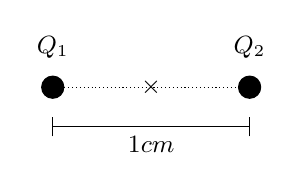
\begin{tikzpicture}[scale=2.50]
				\draw [densely dotted](0,1)--(1,1);
				\draw (0,0.8)--(1,0.8) node [below, pos=0.5] {\small \( 1 \unit{cm}\)};
				\draw (0,0.75)--(0,0.85);
				\draw (1,0.75)--(1,0.85);
				\draw [fill] (0,1) circle[radius=1.6pt];
				\node (c) at (1,1.2) {\small \( Q_2 \)};
				\node (c) at (0,1.2) {\small \( Q_1 \)};
				\node (c) at (0.5,1) {\small \( \times \)};
				\draw [fill] (1,1) circle[radius=1.6pt];
			\end{tikzpicture}\\
			\end{minipage}	
		\end{multicols}
	\tcbline
		\item \( d = 0.07 \unit{m};\quad r = \tfrac{d}{2};\quad h = \sqrt{3} r;\quad Q_1 = Q_3 = Q;\quad Q_2 = -Q \)
		\begin{multicols}{2}
			\begin{flalign*}
				\vec{F_1} &= k \tfrac{q Q_1}{r^2} \vector{-1 \\ 0} &&\\
				\vec{F_2} &= k \tfrac{q Q_2}{r^2} \vector{1 \\ 0} &&\\
				\vec{F_3} &= k \tfrac{q Q_3}{h^2} \vector{0 \\ -1} &&\\
				\vec{F}_{ges} &= \vec{F_1} + \vec{F_2} + \vec{F_3} = \dl{\vector{-0.12 \\ 0.020} \unit{N}} &&
			\end{flalign*}
		\columnbreak
			\begin{minipage}[c][0.7\linewidth][b]{0.5\linewidth}
			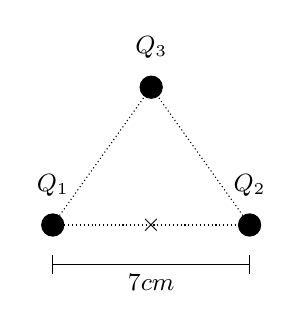
\begin{tikzpicture}[scale=2.50]
				\draw [densely dotted](0,1)--(1,1);
				\draw [densely dotted](0,1)--(0.5,1.7);
				\draw [densely dotted](1,1)--(0.5,1.7);
				\draw (0,0.8)--(1,0.8) node [below, pos=0.5] {\small \( 7 \unit{cm}\)};
				\draw (0,0.75)--(0,0.85);
				\draw (1,0.75)--(1,0.85);
				\draw [fill] (0,1) circle[radius=1.6pt];
				\draw [fill] (1,1) circle[radius=1.6pt];
				\draw [fill] (0.5,1.7) circle[radius=1.6pt];
				\node (c) at (1,1.2) {\small \( Q_2 \)};
				\node (c) at (0,1.2) {\small \( Q_1 \)};
				\node (c) at (0.5,1.9) {\small \( Q_3 \)};
				\node (c) at (0.5,1) {\small \( \times \)};
			\end{tikzpicture}\\
			\end{minipage}	
		\end{multicols}
	\tcbline
		\item \( d = 0.03 \unit{m};\quad r = \tfrac{d}{2};\quad s = \sqrt{5} r;\quad Q_1 = Q_3 = Q;\quad Q_2 = Q_4 = -Q \)
		\begin{multicols}{2}
			\begin{flalign*}
				\vec{F_1} &= k \tfrac{q Q_1}{s^2} \vector{d \\ r} \frac{1}{s} &&\\
				\vec{F_2} &= k \tfrac{q Q_2}{r^2} \vector{0 \\ 1} &&\\
				\vec{F_3} &= k \tfrac{q Q_3}{r^2} \vector{0 \\ -1} &&\\
				\vec{F_4} &= k \tfrac{q Q_4}{s^2} \vector{d \\ -r} \frac{1}{s} &&\\
				\vec{F}_{ges} &= \vec{F_1} + \vec{F_2} + \vec{F_3} = \dl{\vector{0 \\ 0.58} \unit{N}} &&
			\end{flalign*}
		\columnbreak
			\begin{minipage}[c][0.75\linewidth][b]{0.5\linewidth}
			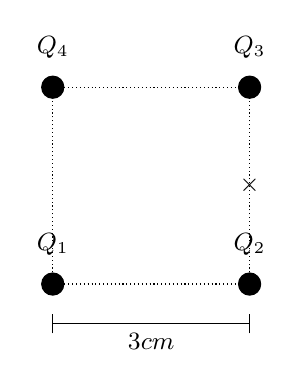
\begin{tikzpicture}[scale=2.50]
				\draw [densely dotted](0,1)--(1,1);
				\draw [densely dotted](0,1)--(0,2);
				\draw [densely dotted](1,1)--(1,2);
				\draw [densely dotted](0,2)--(1,2);
				\draw (0,0.8)--(1,0.8) node [below, pos=0.5] {\small \( 3 \unit{cm}\)};
				\draw (0,0.75)--(0,0.85);
				\draw (1,0.75)--(1,0.85);
				\draw [fill] (0,1) circle[radius=1.6pt];
				\draw [fill] (1,1) circle[radius=1.6pt];
				\draw [fill] (0,2) circle[radius=1.6pt];
				\draw [fill] (1,2) circle[radius=1.6pt];
				\node (c) at (1,1.2) {\small \( Q_2 \)};
				\node (c) at (0,1.2) {\small \( Q_1 \)};
				\node (c) at (0,2.2) {\small \( Q_4 \)};
				\node (c) at (1,2.2) {\small \( Q_3 \)};
				\node (c) at (1,1.5) {\small \( \times \)};
			\end{tikzpicture}\\
			\end{minipage}	
		\end{multicols}
	\end{enumerate}
\end{mybox}


\begin{mybox}{2. Sonnenwind und Ladungsneutralität}
	\centering \( m = 10^{16}\unit{kg};\quad k = \tfrac{1}{4\pi \epsilon_0};\quad \vec{F} = k \tfrac{q_1 q_2}{r^2}\ \vec{r} \)
	\tcblower
	\begin{enumerate}
		\item \( d = 1 \unit{AU};\quad a = r_{Earth};\quad r = \sqrt{d^2 + a^2};\quad \theta_0 = \arctan(\tfrac{a}{d}) \)
		\begin{multicols}{2}
			\begin{flalign*}
				A &= 4\pi d^2 &&\\
				O &= 2\pi r^2 \left( 1-\cos(\theta_0)+\tfrac{1}{2}\sin[2](\theta_0)\right)  &&\\
				\tfrac{O}{A} &= \tfrac{r^2 \left( 1-\cos(\theta_0)+\tfrac{1}{2}\sin[2](\theta_0)\right)}{2d^2} = 9.1 * 10^{-10} &&\\
				M &= m \tfrac{O}{A} = \dl{9.1 * 10^{6} \unit{kg}} &&
			\end{flalign*}
		\columnbreak
			\begin{minipage}[b]{0.5\linewidth}
				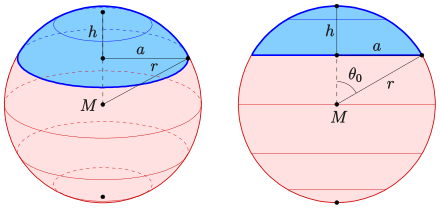
\includegraphics[scale=0.4]{Sphere} 
			\end{minipage}
		\end{multicols}
	\tcbline
		\item \( m_P = m_{Proton};\quad q_e = q_{elementary};\quad m_a = m_{Earth} \)
		\begin{flalign*}
			N &= \tfrac{M}{m_P} &(\text{Amount of Protons}) &&\\
			Q &= N q_e &(\text{Total Charge of Protons}) &&\\
			F_C &= k \tfrac{Q^2}{d^2} &(\text{Coulomb Force felt by Earth}) &&\\
			a_{\perp} &= \tfrac{F_C}{m_a} &(\text{Centripetal Accel. felt by Earth}) &&\\
			T &= 2\pi \sqrt{\tfrac{d}{a_{\perp}}} = \dl{7.03 * 10^7 \unit{s}} & &&
		\end{flalign*}
	\tcbline
		\item If the solar wind consisted of electrons the observed effect would be the same, only of an entirely different order of magnitude, as the mass of an electron is \( 10^{10} \) times smaller than the protons mass. Performing the same calculations outlined above I come to the conclusion that a purely electron-based stream of particles would lead to an orbital period of just over 10 h 30 min. Thank god we have a magnetic field shielding us ...
	\end{enumerate}
\end{mybox}


\begin{mybox}{3. Millikan Versuch}
	\centering \( r = 1.64 * 10^{-6} \unit{m};\quad \rho = 851 \unit{kg/m^3} \)
	\tcblower
	\begin{enumerate}
		\item \( V_{Sphere} = \tfrac{4}{3}\pi r^3;\quad m = V*\rho \)
		\begin{flalign*}
			m &= \tfrac{4}{3}\pi r^3 \rho = \dl{1.57 * 10^{-14}\unit{kg}} &&
		\end{flalign*}
	\tcbline
		\item \( E_0 = \tfrac{F_C}{q} = 1.92 \unit{N/C};\quad F_G = mg  \)
		\begin{flalign*}
			F_G &= F_C &&\\
			q &= \tfrac{mg}{E_0} &&\\
			&= 8.03 * 10^{-14} \unit{C} = \dl{5.01 * 10^{5} q_e} &&
		\end{flalign*}
	\end{enumerate}
\end{mybox}




\end{document}